\section{Evaluation}

We evaluated the timing compartments architecture using the gem5 architectural 
simulator~\cite{gem5} integrated with the DRAMSim2~\cite{DRAMSim2} 
memory simulator. Our experiments use multiprogram workloads 
comprised of SPEC2006 benchmarks compiled for the ARM ISA. 

Table~\ref{tab:config} shows our system configuration.
The cores use the gem5 ``O3`` out-of-order core model which runs at 2GHz. 
Each core has private 32KB L1 instruction and data caches, and private 256KB L2 
cache. The cores share a 4MB L3 cache. We derived cache configuration 
parameters from the Intel Xeon E3-1220L, which is a two core architecture used 
by Amazon EC2. In DRAMSim2, we simulate a 667MHz 2GB DDR3 memory. The 
interconnects in the simulator runs at 1GHz. Unless specified otherwise, each experiment is 
fastforwarded for 1 billion instructions, and run for 100 million 
instructions. We will first describe our security evaluation and then show
the performance evaluation.

\begin{table}
    \caption{Simulator configuration parameters.}
    \centering
    \begin{tabular}{|l|l|l|r|}
        \hline
        \multicolumn{3}{|l|}{gem5 core model} & ``O3''        \\\hline
        \multicolumn{3}{|l|}{CPU Clock}    & 2GHz             \\\hline
        \hline
        \multicolumn{2}{|l|}{Memory}             & 2GB    & 667MHz  \\\hline
        \hline
        \multicolumn{3}{|l|}{Network Clock}      & 1GHz \\\hline
        \hline
        L1d / L1i  & 32kB   & 2-way  & 2 cycles\\\hline
        L2         & 256kB  & 8-way  & 7 cycles \\\hline
        L3         & 4MB    & 16-way & 17 cycles  \\\hline
    \end{tabular}
    \label{tab:config}
\end{table}

\subsection{Security Evaluation}

To experimentally evaluate the security of the timing channel protection in our 
architecture, we use a two-core system with two timing compartments, TC0 and
TC1, running concurrently. The protection policy is configured to disallow any 
timing channels between the two compartments. If the number of cycles required 
to execute a certain number of instructions for a particular benchmark running on 
TC0 depends on which benchmark is running on TC1, it indicates timing 
interference exists that can be exploited to leak information about TC0. A 
secure system should guarantee the benchmark running in TC0 always uses the 
same number of cycles to finish regardless of which benchmark TC1 is running. 

Using the rule above, we evaluated the security of our architecture by running 
a fixed benchmark on TC0 while varying the benchmark on TC1. Then we compared 
the total execution time for the fixed benchmark in different runs. We 
evaluated our architecture as well as the baseline insecure architecture which 
does not implement any protection. As expected, the results for the baseline 
show the execution time of a particular benchmark on Core 0 changes significantly 
depending on the benchmark on Core 1, indicating timing channels exist between
the two cores. On the other hand, when running each pair of benchmarks with 
timing channel protection we observed no execution time difference by changing 
which program runs concurrently with TC0.

\subsection{Time Slice Coordination}
\label{sec:eval_coord}
We analyzed this scheduling problem using our own simulator.
Turns are allocated for each timing compartment in a repeated 
sequence (e.g. 1,2,3,4,1,2,3,4, for four timing compartments). Therefore, a 
schedule repeats after the least common multiple of each 
turn length in the path multiplied by the number of timing compartments. Given 
the turn lengths and offsets of each device, the latency of a request can be 
determined based on the cycle in which a request arrives in the schedule.
The simulator finds each possible latency in a schedule, and calculates the 
expected value of this latency assuming the arrival time at the L2-L3 bus is 
uniform random.

Using this simulator, we exhaustively searched for the optimal L3 hit path 
schedule with the parameters $t_{req}=1,t_{resp}=9,t_{L3}=9$. The 
search space includes turn lengths from 1-25 cycles and all possible offsets 
for each turn length. We confirmed that the intuitive schedule described in 
Section \ref{sec:coordination} achieves the highest L3 hit latency expected value.
Fixing the turn lengths to the optimal ones and adjusting only the offsets,
the worst case latency is 19.6\% worse than the optimal schedule, showing
that coordinating the hit path is important.

Any reasonable L3 miss path search space is far too large to search 
exhaustively. Instead we used integer linear programming optimization 
techniques. Changing a turn length or offset slightly can drastically affect 
the performance, so the search space has many relative minima. We used 
our own simulated annealing optimizer to avoid getting stuck at relative minima 
and increase our chances of finding a global minimum. We optimized for both the 
minimum L3 miss latency and the minimum L2 miss latency assuming a hit rate of 
90\%. 

We initialized the optimizer with a scheme we thought would perform well. The 
optimizer did find a better schedule that improved the miss latency by 5\%. 
After modifying this schedule slightly based on our own reasoning we saw 
further improvement, and re-ran the optimizer. The optimizer did not find a 
better schedule after 20,000 iterations. Using the optimal turn lengths and 
sweeping the space of offsets, the worst-case schedule performed 2.38X worse 
than the optimal schedule.

Optimizing for the L2 miss rate overall is a harder problem since improving the 
consistency of the schedule requires increasing either the L3 hit or miss 
latency so that the least common multiple of the turn lengths is reduced. The 
schedule produced by the optimizer was not one that made any intuitive sense. 
However, the optimal schedule was 8.67X better than the worst case schedule 
with the same turn lengths.

The results for schedule selection study are summarized in Table 
\ref{tab:coord_results}. Overall, scheduling 
interdependent time multiplexed devices is a challenging problem, but the gap 
between the worst and optimal cases show that it is important.

\begin{table}
    \caption{Scheduling Selection Study Results.}
    \centering
    \begin{tabular}{|l|l|l|l|}
        \hline
        \multicolumn{1}{|l|}{Optimized Quantity} & Search & Min & Max \\\hline
        \multicolumn{1}{|l|}{L3 Hit Latency} & Exhaustive & 25.5 & 30.5 \\\hline
        \multicolumn{1}{|l|}{L3 Miss Latency} & Simulated Annealing& 139.5 & 334.5 \\\hline
        \multicolumn{1}{|l|}{L2 Miss Latency} & Simulated Annealing& 38.6 & 344.5 \\\hline
    \end{tabular}
    \label{tab:coord_results}
\end{table}

\subsection{Performance Evaluation}

The timing compartment architecture extends the insecure baseline with
static partitioning and time multiplexing to secure the shared hardware 
resources. These changes lead to underutilization, and thus, a performance
overhead. To evaluate the performance overhead, we ran pairs of
SPEC2006 benchmarks, and measured the execution time of the benchmark
in TC0. Since the timing channel protection mechanisms primarily affect the memory 
hierarchy, the memory intensity of the benchmarks is related to the performance 
overhead.
The memory intensity of each benchmark, in memory requests per thousand 
instructions, during the program segment used for our experiments is shown in
Figure~\ref{fig:memstudy}. Of the SPEC2006 benchmarks, mcf has the most memory 
requests, while astar has none after fast-forwarding for 1B instructions.

For the baseline architecture, we calculate the average execution time of the 
benchmark on Core 0 by averaging among runs with different benchmarks on Core 1. 
The execution time of the benchmark in Core 0 is impacted by the benchmark in 
Core 1. In the timing compartments architecture, the execution time of TC0 (on 
Core 0) is independent of workloads running in other timing compartments.

\begin{figure}
    \begin{center}
        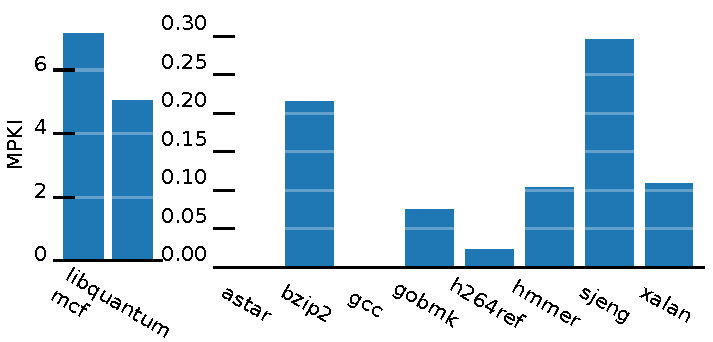
\includegraphics[width=3.4in]{figs/mpki_merged.pdf}
        \caption{Memory intensity of SPEC2006 benchmarks.}
        \label{fig:memstudy}
    \end{center}
\end{figure}

Figure~\ref{fig:performance} shows the performance overhead of full system 
protection as well as the overhead incurred by the changes to the memory 
controller (mc), the cache (waypart), the L3 to memory bus (membus), and the L2 
to L3 bus (L2L3) individually compared to the insecure baseline. The
overheads for libquantum and mcf, which are particularly memory intensive, are 
highest at 69\% and 18\% respectively. However, the arithmetic mean of the 
total overhead is quite low at roughly 9\%. Memory controller protection incurs 
by far the most overhead suggesting the impact on memory bandwidth is more 
significant than bus or cache underutilization. Overall, the results show that 
the timing compartments are viable for applications that require high assurance 
for software isolation.

\begin{figure}
    \begin{center}
        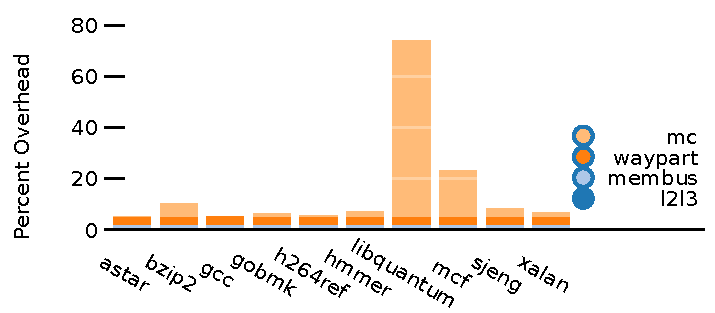
\includegraphics[width=3.4in]{figs/breakdown.pdf}
        \caption{Performance overhead for 2 TCs.}
        \label{fig:performance}
    \end{center}
\end{figure}

The performance overhead is likely to increase as the number of timing 
compartment scales up. To study the impact of the number of timing 
compartments, we evaluated the performance overhead with three and four timing 
compartments on a 4-core  processor, each occupying one core and private L1 and 
L2 caches. They share a 4MB L3 cache. We do not evaluate all permutations of 4 
benchmarks. Instead, we only evaluate the subset of these permutations where 
TC1, TC2, and TC3 are executing the same benchmark. As before, each of these 
workloads with the same program in TC0 is averaged.

The performance overhead as the number of timing compartments increases is 
shown in Figure~\ref{fig:scalability}. The arithmetic mean of the overheads for 
each benchmark for 2, 3 and 4 timing compartments are 9\%, 17\%, and 24\% 
respectively. For libquantum which is particularly memory intensive, the 
overheads are 76\%, 140\%, and 184\% for 2, 3, and 4 timing compartments. The 
results suggest that the overhead of timing timing channel protection is rather 
insensitive to the number of timing compartments for compute-bound 
applications. For memory-intensive applications, the overhead can increase 
noticeably. However, the results still suggest that timing compartments can 
allow distrusting software entities to share hardware and provide better 
overall performance than running them on separate dedicated machines.

\begin{figure}
    \begin{center}
        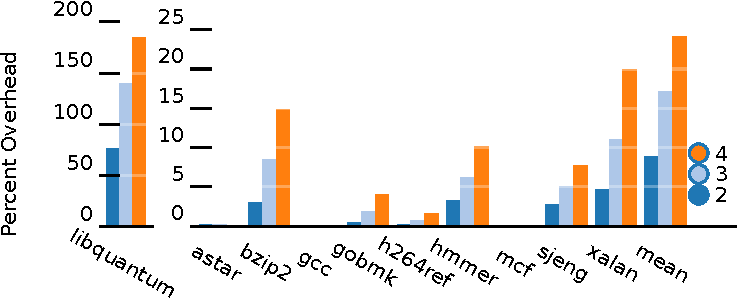
\includegraphics[width=3.4in]{figs/scalability_split.pdf}
        \caption{Performance overhead for 4 TCs.}
        \label{fig:scalability}
    \end{center}
\end{figure}

While future multi-core systems are likely to have a large number of processing 
cores, we note that many security applications will not require many timing 
compartments to be used concurrently. For example, the BYOD application only 
requires two TCs no matter how many cores exist in the system. Similarly, in 
a high-assurance cloud computing environment, the cloud provider can limit the
number of high-assurance virtual machines that can be located on each physical
system while increasing the system utilization by co-locating non-secure
virtual machines with high-assurance ones.

\subsection{Cache Coherence Performance Overhead}
Adding the timing channel protection for snooping bus can introduce some performance overhead. We evaluate some 
splash2~\cite{splash2} benchmarks in gem5. The system we model is the one shown in Figure~\ref{fig:coherent_system}.
We use the same splash2 benchmarks for Attacker0 and Attacker1, each consists of two threads. We terminate the simulation
when thread on core 0 reaches 100M instructions. 
Our baseline is a system where every other timing channel protection scheme we proposed is implemented except for the snooping bus.
We then compare it with the system where the snooping bus is also protected. This comparison enables us to quantify the exact overhead introduced by adding cache coherence protection. 

The results are shown in Figure~\ref{fig:splash2}. As can be seen, the overhead of adding cache coherence protection is
quite low, with the highest overhead less than 1.5\%. In some cases the protection scheme even outperform the baseline, 
mainly because the round-robin scheduling may have avoided some snooping bus contention in the baseline scheduling. 
The main reason for the low overhead is that the coherent traffic is quite rare in programs, hence the round-robin
snooping bus will not cause much overhead to the overall program execution time.

\begin{figure}
    \begin{center}
        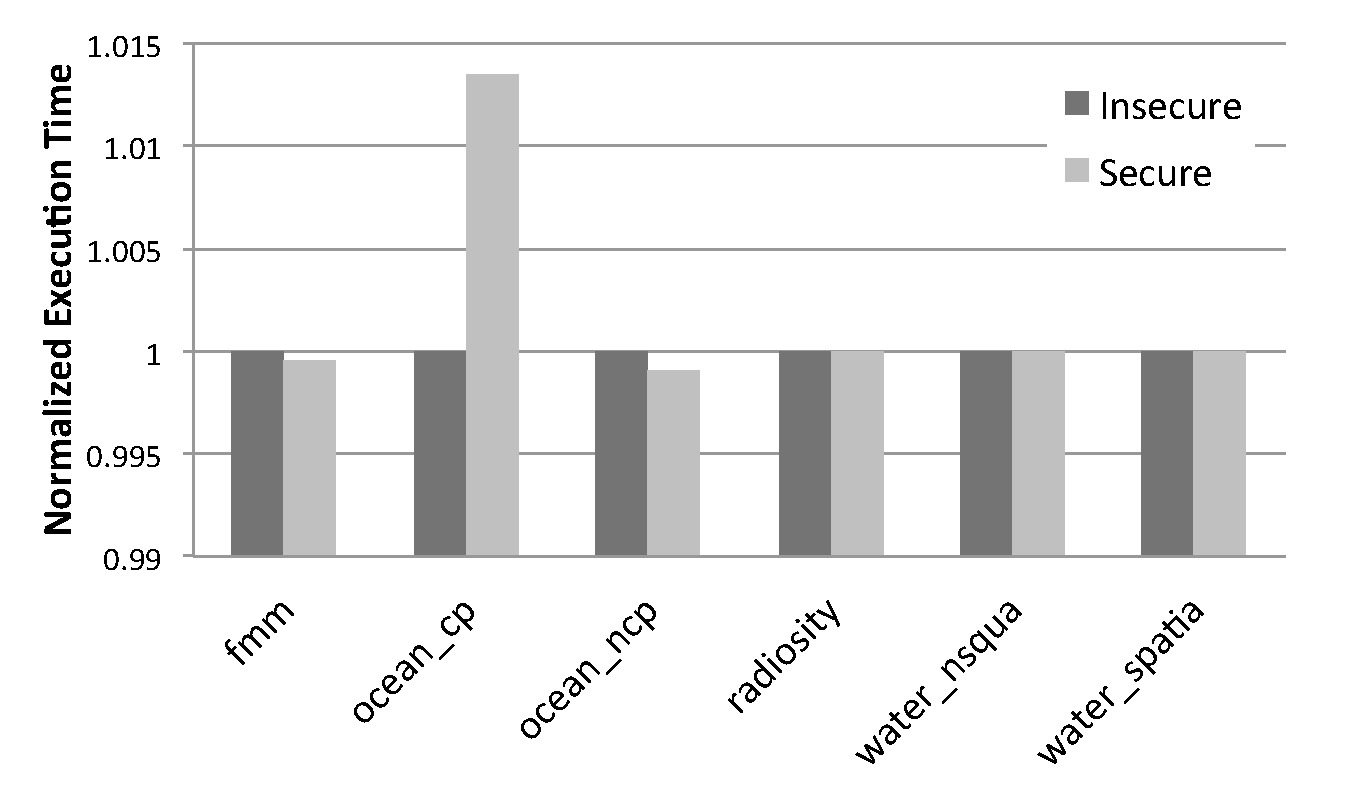
\includegraphics[width=2.79in]{figs/splash2.pdf}
        \caption{Performance Overhead of Cache Coherence Protection}
        \label{fig:splash2}
    \end{center}
\end{figure}
